\documentclass[11pt,a4paper]{article}

% Typeface: XeLaTeX with Latin Modern Roman (fontspec default)
\usepackage{fontspec}
\usepackage{polyglossia}
\setdefaultlanguage{turkish}

% Page: the measures of the note template (A4, 11 pt, 4.5 cm side margins, header and page count)
\usepackage[a4paper,left=4.5cm,right=4.5cm,top=4.5cm,bottom=4.1cm,headheight=14pt,headsep=0.55cm,
  footskip=0.55cm]{geometry}
\linespread{0.946}
\usepackage{fancyhdr}
\usepackage{lastpage}
\pagestyle{fancy}
\fancyhf{}
\fancyhead[L]{\small\textbf{PROJE NOTU} $|$ LCG in R}
\fancyhead[R]{\small\textbf{Derlenme tarihi:} \today}
\fancyfoot[C]{\small\thepage\,/\,\pageref{LastPage}}
\renewcommand{\headrulewidth}{0.4pt}

\usepackage{microtype}
\usepackage{amsmath,amssymb}
\usepackage{booktabs,array,tabularx}
\usepackage{graphicx}
\usepackage{enumitem}
\setlist{noitemsep, topsep=3pt, leftmargin=*}
\usepackage{xcolor}
\definecolor{secblue}{HTML}{1F3A5F}
\definecolor{boxback}{HTML}{EEF2F6}
\definecolor{mark}{HTML}{9B2226}
\definecolor{hl}{HTML}{FFF36B}
\usepackage{titlesec}
\titleformat{\section}{\color{secblue}\bfseries\normalsize}{\thesection.}{0.4em}{}
\titlespacing*{\section}{0pt}{10pt}{4pt}
\usepackage[font=small,labelfont=bf,labelsep=period,skip=4pt]{caption}
\usepackage[bottom]{footmisc}
\captionsetup[figure]{name=Şekil}
\captionsetup[table]{name=Tablo}
\setlength{\parindent}{0pt}
\setlength{\parskip}{5pt}
\setlength{\textfloatsep}{10pt}
\emergencystretch=3em

\newcommand{\ExOnePeriod}{56.826}
\newcommand{\ExOneShare}{0{,}72}
\newcommand{\ExTwoTail}{2}
\newcommand{\ExTwoPeriod}{14.076}
\newcommand{\ExTwoShare}{0{,}14}
\newcommand{\ExTwoGcd}{3}
\newcommand{\ExThreePeriod}{8}
\newcommand{\VOneStepTwo}{14.079}
\newcommand{\ReadmeStated}{27, 9, 3, 1, 11, 23, 29}
\newcommand{\ReadmeComputed}{27, 9, 3, 1, 11, 25, 19, 17, 27}
\newcommand{\NuOne}{1079{,}0}
\newcommand{\NuOneNorm}{0{,}357}
\newcommand{\NuOneSpacing}{0{,}00093}
\newcommand{\NuTwo}{1722{,}0}
\newcommand{\NuTwoNorm}{0{,}508}
\newcommand{\NuTwoSpacing}{0{,}00058}
\newcommand{\BatteryN}{10.000}
\newcommand{\BatteryTests}{36}
\newcommand{\BatteryExpectedFalse}{0{,}36}
\newcommand{\BatteryRejections}{0}
\newcommand{\BatteryMinP}{0{,}029}
\newcommand{\BatteryMinPGen}{Mersenne-Twister (R)}
\newcommand{\SerialN}{300.000}
\newcommand{\RanduChi}{80.064}
\newcommand{\SerialDf}{7.999}
\newcommand{\RanduTriples}{299.998}
\newcommand{\RanduPlanes}{15}
\newcommand{\RanduPlaneMin}{-5}
\newcommand{\RanduPlaneMax}{9}
\newcommand{\PerfCycleSize}{32.768}
\newcommand{\PerfCycleVOne}{2{,}14}
\newcommand{\PerfCycleVTwo}{0{,}018}
\newcommand{\PerfCycleRatio}{120}
\newcommand{\PerfCycleMax}{16.777.216}
\newcommand{\PerfCycleMaxTime}{8{,}9}
\newcommand{\PerfGenVOne}{0{,}69}
\newcommand{\PerfGenVTwo}{0{,}16}
\newcommand{\PerfGenRatio}{4{,}3}
\newcommand{\PerfMachine}{R 4.5.1}
\newcommand{\SlopeVOne}{2{,}03}
\newcommand{\SlopeVTwo}{0{,}99}


\begin{document}


\vspace*{14pt}
\begin{tabular}{@{}p{2.35cm}@{}p{\dimexpr\textwidth-2.35cm}@{}}
\textbf{BAŞLIK:} & \textbf{\large Doğrusal eşlik üreteci (LCG): periyot, kafes yapısı ve ampirik testler}\\[3pt]
\textbf{KONU:} & \texttt{linear-congruential-generator} deposunun 2.\ sürümündeki analizlerin amacı, yöntemi ve sonuçları\\[3pt]
\textbf{YAZAR:} & Muhammed İkbal Yılmaz (myucanlar@gmail.com)
\end{tabular}

\vspace{8pt}
\vspace{12pt}

\section{Amaç ve kapsam}

Doğrusal eşlik üreteci (linear congruential generator, LCG) bir tohum $x_0$'dan başlayarak
\[
  x_{n+1} = (a\,x_n + c) \bmod m, \qquad u_n = x_n/m \in [0,1)
\]
dizisini üretir; $a$ çarpan, $c$ artım, $m$ modüldür. Dizi tamamen belirlenimlidir, bu yüzden bir üretecin iyi olup olmadığı
iki soruya indirgenir: \emph{kaç sayı üretebilir} (periyot) ve \emph{ardışık sayılar ne kadar bağımsız görünür} (kafes yapısı
ve testler). Bu notta dört analiz var; her biri bu sorulardan birine yanıt verir:

\begin{enumerate}
  \item \textbf{Periyot:} Üreteç kendini tekrar etmeden önce kaç sayı verir?
  \item \textbf{Kafes yapısı:} Ardışık sayı çiftleri birim karede nasıl dağılır?
  \item \textbf{Ampirik testler:} Klasik testler 1.\ ve 2.\ analizde görülen zayıflıkları yakalayabilir mi?
  \item \textbf{Çalışma süresi:} Yeni kod, 1.\ sürümün sınırlarını gerçekten kaldırıyor mu?
\end{enumerate}

İncelenen altı üreteç bilinçli seçildi: 1.\ sürümün üç örneği (asıl inceleme konusu) ile literatürden üç karşılaştırma noktası.
\textbf{RANDU} ($a=65539$, $c=0$, $m=2^{31}$) kusuru iyi bilinen bir üreteçtir ve testlerin bu kusuru bulup bulamadığını sınamak
için kullanılır. \textbf{MINSTD} ($a=16807$, $c=0$, $m=2^{31}-1$) Park ve Miller'ın (1988) önerdiği en uzun periyotlu çarpımsal
üreteçtir. \textbf{rand48 parametreleri} ($a=25.214.903.917$, $c=11$, $m=2^{48}$) çarpımın R'ın sayı duyarlılığını aştığı durumu
temsil eder. LCG olmayan \textbf{Mersenne-Twister} (R'ın varsayılan üreteci; Matsumoto ve Nishimura, 1998) testlerde ölçüt olarak
kullanıldı.

\section{Yöntem}

Kod yalnızca temel R kullanır. Her sonuç birim testlerinde bağımsız bir hesapla (kaba kuvvet araması, düz döngü ya da tam sayı
aritmetiğiyle hesaplanmış referans değerler) karşılaştırılmıştır.

\begin{itemize}
  \item \textbf{Kesin aritmetik.} R sayıları çift duyarlıklı tutar; $2^{53}$'e kadar her tam sayı kesin temsil edilir. $a\,x_n$
  bu sınırı aşınca sonuç sessizce yanlış olur. rand48 parametreleriyle doğrudan hesap, ikinci değerde kesin diziden ayrılır. Bu
  nedenle $a$, $2^s$ tabanında basamaklarına ayrılır ve $a x \bmod m$ Horner yöntemiyle, hiçbir ara değer $2^{53}$'e ulaşmadan
  hesaplanır. Yöntem $m \le 2^{51}$ için kesindir.
  \item \textbf{İleri atlama.} $k$ adım sonra da dönüşüm doğrusaldır: $x_{n+k} = (A_k x_n + C_k) \bmod m$. $(A_k, C_k)$ ikili
  üs alma ile $O(\log k)$ adımda bulunur (Brown, 1994). Sayılar $\sqrt{n}$ uzunluğunda bloklar halinde üretilir; her blok bir
  öncekinden tek bir vektör işlemiyle elde edilir.
  \item \textbf{Kuyruk ve döngü.} Sonlu durum uzayında her dizi önce $\mu$ uzunluğunda bir kuyruktan geçer, sonra $\lambda$
  uzunluğunda bir döngüye girer. Brent (1980) algoritması $\lambda$'yı sabit bellekle bulur, $\mu$ ileri atlamayla gelir. 1.\
  sürüm her yeni değeri önceki tüm değerlerle karşılaştırıyordu; bu $O((\mu+\lambda)^2)$ işlem demektir ve yalnızca
  $\mu+\lambda$'yı verir.
\end{itemize}

\section{Analiz 1: Periyot (Tablo~\ref{tab:periyot})}

\textbf{Neden.} Periyot, bir üreteçten kullanılabilecek en fazla sayıdır. Periyottan uzun bir örnek aynı sayıları aynı sırayla
tekrar eder; bu durumda simülasyon sonuçları bağımsız gözlemlere dayanmaz. Periyot örneklemle tahmin edilmez, teoriyle kesin
hesaplanır.

\textbf{Yöntem.} $c \ne 0$ ise Hull--Dobell teoremi geçerlidir. Teoreme göre periyot her tohum için $m$'ye ancak ve ancak şu üç
koşul sağlanırsa eşittir: (i) $c$ ile $m$ aralarında asaldır, (ii) $a-1$, $m$'nin her asal çarpanına bölünür, (iii) $m$ 4'e
bölünüyorsa $a-1$ de 4'e bölünür (Hull ve Dobell, 1962). $c=0$ durumunu teorem kapsamaz. Bu durumda $m$ ile aralarında asal
bir tohum için periyot, $a$'nın $m$ modülüne göre mertebesidir; bu mertebe en fazla Carmichael fonksiyonu $\lambda(m)$ kadar
olabilir (Knuth, 1997, §3.2.1.2). Teorinin doğrudan yanıt vermediği durumlarda Brent algoritması kullanıldı.

\begin{table}[h]
\centering\footnotesize\setlength{\tabcolsep}{4pt}
\caption{Hull--Dobell koşulları ile kuyruk ve döngü uzunlukları (tohum $x_0=1$; 3.\ örnekte $x_0=27$). Koşullar yalnızca
$c\ne0$ için gösterilmiştir.}\label{tab:periyot}
\scriptsize\setlength{\tabcolsep}{1.8pt}
\resizebox{\textwidth}{!}{%
\begin{tabular}{@{}>{\raggedright\arraybackslash}p{1.8cm}rrlccccr>{\raggedright\arraybackslash}p{1.45cm}@{}}
\toprule
 & & & & \multicolumn{3}{c}{Hull--Dobell} & & & \\
\cmidrule(lr){5-7}
Üreteç & $a$ & $c$ & $m$ & (i) & (ii) & (iii) & Kuyruk & Döngü & Yöntem \\
\midrule
Sürüm 1, örnek 1 & 1.079 & 863 & $7\cdot 11\cdot 19\cdot 5413$ & evet & hayır & evet & 0 & 56.826 & Brent \\
Sürüm 1, örnek 2 & 1.722 & 990 & $3^{2}\cdot 13\cdot 139\cdot 613$ & hayır & hayır & evet & 2 & 14.076 & Brent \\
Sürüm 1, örnek 3 & 11 & 0 & $2^{5}$ & -- & -- & -- & 0 & 8 & $a$'nın mertebesi \\
RANDU & 65.539 & 0 & $2^{31}$ & -- & -- & -- & 0 & $2^{29}$ & $a$'nın mertebesi \\
MINSTD (Park--Miller) & 16.807 & 0 & $2^{31}-1$ & -- & -- & -- & 0 & $2^{31}-2$ & $a$'nın mertebesi \\
rand48 parametreleri & 25.214.903.917 & 11 & $2^{48}$ & evet & evet & evet & 0 & $2^{48}$ & Hull--Dobell \\
\bottomrule

\end{tabular}}
\end{table}

\textbf{Bulgu ve yorum.} 1.\ sürümün iki büyük örneğinin döngüleri yalnızca \ExOnePeriod{} ve \ExTwoPeriod{} sayıdır; bu,
modüllerinin \%\ExOneShare{} ve \%\ExTwoShare{}'i eder. 1.\ örnekte (ii) sağlanmaz: $a-1 = 1078 = 2\cdot7^2\cdot11$, $m$'nin
çarpanları olan 19 ve 5413'e bölünmez. 2.\ örnekte (i) ve (ii) sağlanmaz. Ayrıca $a$ ile $m$'nin ortak böleni
\ExTwoGcd{} olduğundan dönüşüm bire bir değildir ve dizi döngüye girmeden önce \ExTwoTail{} değerlik bir kuyruktan geçer.
1.\ sürüm bu örnekte \VOneStepTwo{} sonucunu veriyordu; bu sayı kuyruğu ve döngüyü birbirinden ayırmaz. 3.\ örnek
çarpımsaldır ($c=0$); periyodu \ExThreePeriod{}, yani $\lambda(32)$, ulaşılabilecek en büyük değerdir. 1.\ sürümün README'si
bu örnek için \ReadmeStated{} dizisini veriyordu; doğrusu \ReadmeComputed{}'dir. Pratik sonuç: bu iki üreteçten birkaç bin
sayıdan fazlasını kullanan her simülasyon aynı sayıları yeniden kullanır.

\section{Analiz 2: Kafes yapısı (Şekil~\ref{fig:kafes})}

\textbf{Neden.} Uzun periyot tek başına yeterli değildir. LCG'de $u_{n+1}$, $u_n$'nin doğrusal bir fonksiyonudur (mod 1). Bu
yüzden $(u_n, u_{n+1})$ çiftleri birim karede birbirine paralel doğrular üzerine düşer. Doğrular arası boşluk büyüdükçe karenin
geniş bölgeleri hiç ziyaret edilmez.

\textbf{Yöntem.} Spektral test (Knuth, 1997, §3.3.4) bu boşluğu tek bir sayıyla ölçer. $\nu_2$, $s_1 + a s_2 \equiv 0 \pmod m$
koşulunu sağlayan sıfırdan farklı en kısa $(s_1,s_2)$ vektörünün uzunluğudur; komşu doğrular arasındaki en büyük uzaklık
$1/\nu_2$'dir. $\nu_2 \le (4/3)^{1/4}\sqrt{m}$ olduğundan bu üst sınıra oranı 0 ile 1 arasında, ölçekten bağımsız bir
ölçüttür; 1'e yakın olması iyidir (L'Ecuyer, 1999). $(-a, 1)$ vektörü koşulu her zaman sağladığından $\nu_2 \le \sqrt{a^2+1}$
olur: küçük çarpan, doğruların seyrek olması demektir. En kısa vektör Lagrange--Gauss indirgemesiyle bulundu; yöntem
$m \le 2^{26}$ için kesindir.

\textbf{Şekil neden böyle çizildi?} $\nu_2$ tek bir sayıdır; şekil bu sayının ne anlama geldiğini gösterir. Doğrular
yaklaşık 0,001 aralıklı olduğundan birim karenin tamamında görünmezler. Bu yüzden 1.\ örneğin tam bir periyodu (\ExOnePeriod{}
çift) içinden $u_n < 0{,}004$ olanlar gösterildi. Karşılaştırma için aynı sayıda Mersenne-Twister çifti yan panelde yer alır.
Kafes yapısı yoksa noktalar dağınık düşer.

\begin{figure}[h]
\centering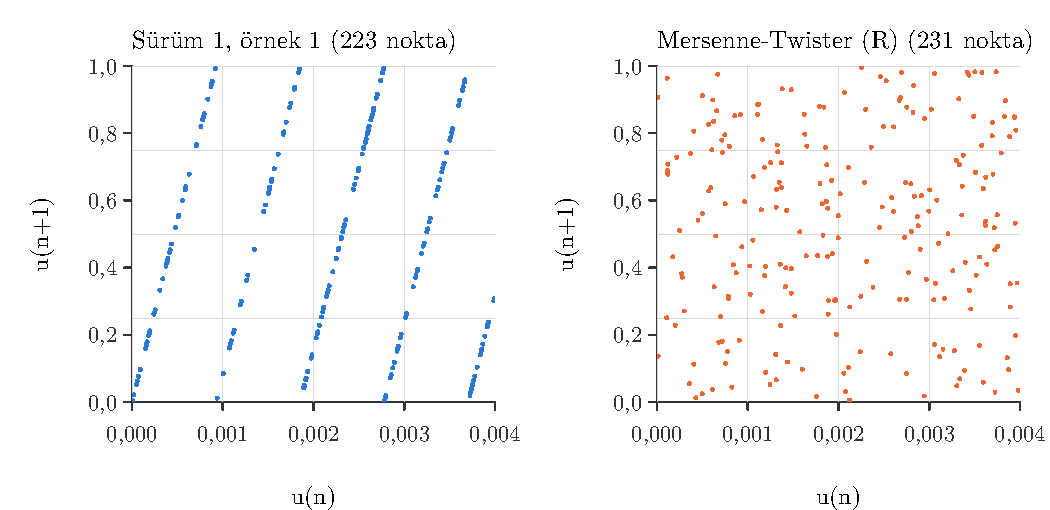
\includegraphics[width=\textwidth]{../figures/tr/fig1_pairs.pdf}
\caption{Ardışık çiftler $(u_n, u_{n+1})$, $u_n < 0{,}004$. Sol: 1.\ sürümün 1.\ örneği, tam periyot. Sağ: aynı sayıda
Mersenne-Twister çifti.}\label{fig:kafes}
\end{figure}

\textbf{Bulgu ve yorum.} 1.\ örnekte $\nu_2 = \NuOne$, doğrular arası uzaklık $\NuOneSpacing$ ve normalize değer $\NuOneNorm$'dür.
2.\ örnekte bu değerler sırasıyla $\NuTwo$, $\NuTwoSpacing$ ve $\NuTwoNorm$'dür. Şekilde sol paneldeki noktalar eğimi $a$ olan
birkaç doğru üzerinde toplanır, sağ panelde ise belirli bir düzen yoktur. Normalize değerin 1'den uzak olması, çarpanın kafes
yapısı açısından kötü seçildiğini gösterir.

\section{Analiz 3: Ampirik testler (Tablo~\ref{tab:test}, Şekil~\ref{fig:randu})}

\textbf{Neden.} Uygulamada üreteçler çoğunlukla istatistiksel testlerle değerlendirilir. Bu analiz testlerin gücünü sınar:
kusuru teoriyle bilinen üreteçlerde (1.\ sürüm örnekleri, RANDU) klasik testler bu kusuru gösterebiliyor mu?

\textbf{Yöntem.} Her üreteçten \BatteryN{} sayı alındı ve altı klasik test uygulandı (Knuth, 1997, §3.3.2): 100 hücrede eşit
dağılım ($\chi^2$), Kolmogorov--Smirnov, örtüşmeyen ikililer ve üçlülerde seri test, gecikme-1 otokorelasyonu ve artan/azalan
koşu testi. Örtüşmeyen gruplar kullanıldı; böylece hücre sayıları multinom dağılır ve $\chi^2$ referans dağılımı geçerli olur.
Anlamlılık düzeyi 0,01'dir. \BatteryTests{} testte, üreteçler kusursuz olsa bile, yaklaşık \BatteryExpectedFalse{} yanlış ret
beklenir. Ardından daha ince bir ızgarayla ($20^3$ hücre) \SerialN{} sayı üzerinde üçlü seri testi yapıldı.

\begin{table}[h]
\centering\footnotesize\setlength{\tabcolsep}{4pt}
\caption{$p$-değerleri. İlk altı sütun: üreteç başına \BatteryN{} sayı. Son sütun: örtüşmeyen üçlüler, $20^3$ hücre,
\SerialN{} sayı.}\label{tab:test}
\scriptsize\setlength{\tabcolsep}{3pt}
\begin{tabular}{@{}>{\raggedright\arraybackslash}p{2.1cm}cccccc>{\raggedright\arraybackslash}p{1.5cm}@{}}
\toprule
 & Eşit & & & & Oto- & & Üçlü, \\
 & dağılım & KS & İkili & Üçlü & korelasyon & Koşu & $20^3$ \\
\midrule
Sürüm 1, örnek 1 & 0{,}843 & 0{,}707 & 0{,}069 & 0{,}477 & 0{,}332 & 0{,}033 & periyot kısa \\
Sürüm 1, örnek 2 & 0{,}645 & 0{,}711 & 0{,}832 & 0{,}215 & 0{,}405 & 0{,}806 & periyot kısa \\
RANDU & 0{,}387 & 0{,}814 & 0{,}578 & 0{,}661 & 0{,}184 & 0{,}351 & $<$0{,}001 \\
MINSTD (Park--Miller) & 0{,}554 & 0{,}695 & 0{,}946 & 0{,}536 & 0{,}960 & 0{,}181 & 0{,}605 \\
rand48 parametreleri & 0{,}643 & 0{,}935 & 0{,}188 & 0{,}676 & 0{,}549 & 0{,}874 & 0{,}593 \\
Mersenne-Twister (R) & 0{,}029 & 0{,}389 & 0{,}688 & 0{,}965 & 0{,}843 & 0{,}312 & 0{,}994 \\
\bottomrule

\end{tabular}
\end{table}

\textbf{Bulgu.} \BatteryTests{} testin hiçbiri 0,01 düzeyinde reddetmedi; en küçük $p$-değeri (\BatteryMinP{}), ölçüt
olarak kullanılan \BatteryMinPGen{}'e aittir. Küçük örneklemli klasik testler 1.\ ve 2.\ analizdeki zayıflıkları göstermedi. İnce
ızgaralı üçlü testte RANDU açıkça reddedildi ($\chi^2 = \RanduChi$, serbestlik derecesi \SerialDf). 1.\ sürümün iki
örneği bu teste giremedi bile, çünkü \SerialN{} sayılık bir örneklem onların döngüsünü birkaç kez tekrar ederdi.

\textbf{Şekil neden çizildi?} Test RANDU'nun üçlülerinin eşit dağılmadığını söyler ama nedenini söylemez. Neden cebirseldir:
$a = 2^{16}+3$ olduğundan $a^2 = 2^{32} + 6\cdot2^{16} + 9 \equiv 6a - 9 \pmod{2^{31}}$ ve dolayısıyla
$9u_k - 6u_{k+1} + u_{k+2}$ her $k$ için bir tam sayıdır. Şekil bu bileşimin dağılımını gösterir. RANDU'da \RanduTriples{}
üçlünün tamamı $\RanduPlaneMin$ ile $\RanduPlaneMax$ arasındaki \RanduPlanes{} tam sayıda toplanır; yani her üçlü birim küpte
\RanduPlanes{} paralel düzlemden birinin üzerindedir (Marsaglia, 1968). Aynı modül büyüklüğündeki MINSTD'de değerler sürekli
yayılır.

\begin{figure}[h]
\centering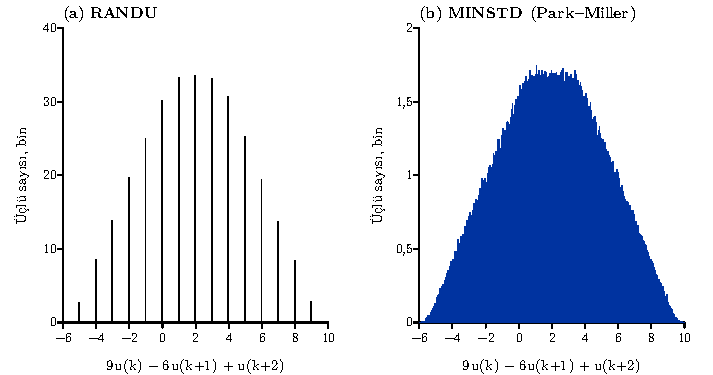
\includegraphics[width=\textwidth]{../figures/tr/fig2_randu_planes.pdf}
\caption{\RanduTriples{} ardışık üçlüde $9u_k - 6u_{k+1} + u_{k+2}$ değerinin histogramı (sütun genişliği 0,05).}\label{fig:randu}
\end{figure}

\textbf{Yorum.} Bir üretecin birkaç testi geçmesi gerekli bir koşuldur, yeterli değildir. Ciddi değerlendirmeler TestU01 gibi
büyük test kümeleriyle yapılır (L'Ecuyer ve Simard, 2007). Bir LCG'nin periyodu ve kafes yapısı ise testle tahmin
edilmeden teoriyle kesin olarak hesaplanabilir.

\section{Analiz 4: Çalışma süresi (Şekil~\ref{fig:sure})}

\textbf{Neden.} 1.\ sürümün tekrar kontrolü, döngü uzunluğunun karesiyle büyüyen bir maliyete sahipti. Bu, analiz edilebilecek
periyotları fiilen sınırlıyordu. Bu analiz, iyileştirmenin ne kadar olduğunu ve nereden geldiğini ölçer.

\textbf{Yöntem.} Hull--Dobell koşullarını sağlayan $x \mapsto (5x+1) \bmod 2^k$ üreteçlerinin döngü uzunluğu tam olarak
$2^k$'dır; böylece problem büyüklüğü kontrol altındadır. Her süre üç ölçümün medyanıdır. Kısa çağrılar zamanlayıcının
çözünürlüğünün altında kalmasın diye her ölçüm en az 0,2 saniye sürecek kadar tekrarlandı.

\textbf{Şekil nasıl okunur?} Eksenler logaritmiktir. $n^k$ ile büyüyen bir süre bu eksenlerde eğimi $k$ olan bir doğru olarak
görünür; böylece büyüme mertebesi doğrudan okunur. En küçük kareler eğimi 1.\ sürüm için \SlopeVOne{} (karesel), 2.\ sürüm için
\SlopeVTwo{}'dür (doğrusal).

\begin{figure}[h]
\centering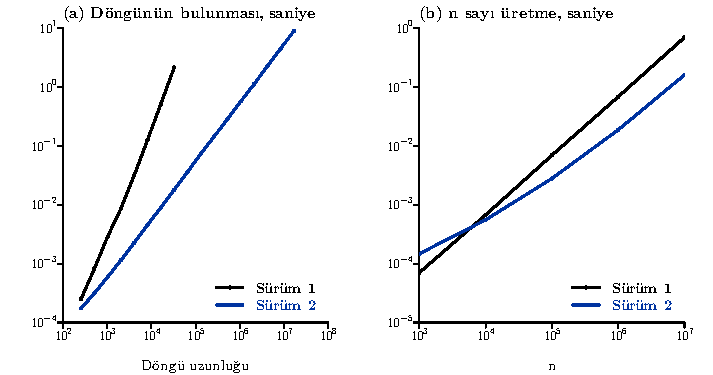
\includegraphics[width=\textwidth]{../figures/tr/fig3_performance.pdf}
\caption{Çalışma süresi, üç ölçümün medyanı (\PerfMachine). Sol: döngünün bulunması (1.\ sürüm yalnızca $2^{15}$'e kadar).
Sağ: $n$ MINSTD sayısının üretilmesi.}\label{fig:sure}
\end{figure}

\textbf{Bulgu.} \PerfCycleSize{} uzunluğundaki bir döngüyü 1.\ sürüm \PerfCycleVOne{} saniyede, 2.\ sürüm \PerfCycleVTwo{}
saniyede bulur (yaklaşık \PerfCycleRatio{} kat). 2.\ sürüm \PerfCycleMax{} uzunluğundaki bir döngüyü \PerfCycleMaxTime{}
saniyede bulur. Sayı üretiminde iki yöntem de doğrusaldır ve fark sabit bir çarpandır: $10^7$ sayı düz döngüyle
\PerfGenVOne{}, blok halinde atlamayla \PerfGenVTwo{} saniye sürer (\PerfGenRatio{} kat). Birkaç bin sayı için düz döngü daha
hızlıdır. Mutlak süreler makineye bağlıdır, büyüme mertebesi bağlı değildir.

\section{Sonuç ve sınırlılıklar}

\begin{itemize}
  \item 1.\ sürümün parametreleri bir ölçüte göre seçilmemişti. Hull--Dobell koşulları, mertebe ve spektral test bu
  parametrelerin zayıflıklarını doğrudan gösterir. Periyottan kısa örneklemlerle yapılan klasik testler göstermez.
  \item $2^{51}$'den büyük modüller (ör. birçok güncel LCG'nin kullandığı $2^{64}$) büyük tam sayı aritmetiği gerektirir ve
  desteklenmez. Spektral test iki boyutlu ve $m \le 2^{26}$ için hesaplanır.
  \item Test kümesi küçüktür; amacı göstermektir, bir üreteci onaylamak değildir. Süreler tek bir makinede ölçülmüştür.
  \item LCG'ler kriptografik amaçlara uygun değildir. Simülasyon için R'ın yerleşik üreteçleri tercih edilmelidir.
\end{itemize}

\section*{Kaynaklar}
{\small
\setlength{\parskip}{2pt}
\hangindent=1.27cm\hangafter=1 Brent, R. P. (1980). An improved Monte Carlo factorization algorithm. \textit{BIT}, 20(2), 176--184.\par
\hangindent=1.27cm\hangafter=1 Brown, F. B. (1994). Random number generation with arbitrary strides. \textit{Transactions of the American Nuclear Society}, 71, 202--203.\par
\hangindent=1.27cm\hangafter=1 Hull, T. E., \& Dobell, A. R. (1962). Random number generators. \textit{SIAM Review}, 4(3), 230--254.\par
\hangindent=1.27cm\hangafter=1 Knuth, D. E. (1997). \textit{The Art of Computer Programming, Vol.\ 2: Seminumerical Algorithms} (3.\ baskı). Addison-Wesley.\par
\hangindent=1.27cm\hangafter=1 L'Ecuyer, P. (1999). Tables of linear congruential generators of different sizes and good lattice structure.
\textit{Mathematics of Computation}, 68(225), 249--260.\par
\hangindent=1.27cm\hangafter=1 L'Ecuyer, P., \& Simard, R. (2007). TestU01: A C library for empirical testing of random number generators.
\textit{ACM Transactions on Mathematical Software}, 33(4), Makale 22.\par
\hangindent=1.27cm\hangafter=1 Marsaglia, G. (1968). Random numbers fall mainly in the planes. \textit{Proceedings of the National Academy of Sciences}, 61(1), 25--28.\par
\hangindent=1.27cm\hangafter=1 Matsumoto, M., \& Nishimura, T. (1998). Mersenne Twister: A 623-dimensionally equidistributed uniform pseudo-random number
generator. \textit{ACM Transactions on Modeling and Computer Simulation}, 8(1), 3--30.\par
\hangindent=1.27cm\hangafter=1 Park, S. K., \& Miller, K. W. (1988). Random number generators: Good ones are hard to find. \textit{Communications of the ACM},
31(10), 1192--1201.\par

\smallskip
Tüm sayılar
\texttt{figures/*.csv} dosyalarından \texttt{make\_paper.R} ile üretilir.
}

\end{document}
